
When a coroutine is started, three things happen:

\begin{itemize}
\item 
A coroutine frame is created to store all necessary data of the coroutine. This usually happens on the heap.

However, compilers are allowed to put the coroutine frame on the stack. This typically happens if the lifetime of the coroutine is within the lifetime of the caller and the compiler has enough information to compute the size of the frame.

\item 
All parameters of the coroutine are copied into the frame.

Note that references are copied as references; it is not that their values are copied. This means that the arguments that the reference parameters refer to have to be valid as long as the coroutine is running.

The advice is to never declare coroutine parameters as references. Otherwise, fatal runtime errors with undefined behavior may occur.

\item 
The promise object is created inside the frame. Its purpose is to store the state the coroutine and provide hooks for customization while the coroutine is running.

You can think of these objects as a “coroutine state controller” (an object that controls the behavior of the coroutine and can be used to track its state).
\end{itemize}

Figure 15.1 visualizes this initialization and shows which customization points of the promise object are used while the coroutine is running.

\begin{center}
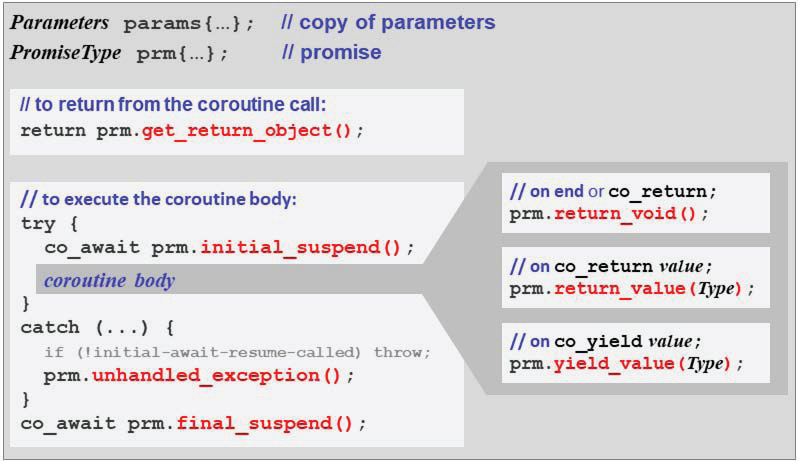
\includegraphics[width=0.8\textwidth]{content/chapter15/images/1.png}\\
Figure 15.1. Coroutine frame and promise
\end{center}

\mySubsubsection{15.2.1}{How Coroutine Interfaces, Promises, and Awaitables Interact}

Let us also bring the awaitables into play again and see how work as a whole is organized:

\begin{itemize}
\item 
For each coroutine started, the compiler creates a promise.

\item 
That promise, embedded in a coroutine handle, is then placed in a coroutine interface. That is, the coroutine interface usually controls the lifetime of the handle and its promise.

\item 
On suspension, coroutines use awaitables to control what happens on suspension and resumption.
\end{itemize}

The following program demonstrates the exact control flow by using a tracing coroutine interface, promise, and awaiter. The tracing coroutine interface and promise are implemented as follows:

\filename{coro/tracingcoro.hpp}

\begin{cpp}
#include <iostream>
#include <coroutine>
#include <exception> // for terminate()

// coroutine interface to deal with a simple task
// - providing resume() to resume it
class [[nodiscard]] TracingCoro {
	public:
	// native coroutine handle and its promise type:
	struct promise_type;
	using CoroHdl = std::coroutine_handle<promise_type>;
	CoroHdl hdl; // coroutine handle
	
	// helper type for state and customization:
	struct promise_type {
		promise_type() {
			std::cout << " PROMISE: constructor\n";
		}
		~promise_type() {
			std::cout << " PROMISE: destructor\n";
		}
		auto get_return_object() { // init and return the coroutine interface
			std::cout << " PROMISE: get_return_object()\n";
			return TracingCoro{CoroHdl::from_promise(*this)};
		}
		auto initial_suspend() { // initial suspend point
			std::cout << " PROMISE: initial_suspend()\n";
			return std::suspend_always{}; // - start lazily
		}
		void unhandled_exception() { // deal with exceptions
			std::cout << " PROMISE: unhandled_exception()\n";
			std::terminate(); // - terminate the program
		}
		void return_void() { // deal with the end or co_return;
			std::cout << " PROMISE: return_void()\n";
		}
		auto final_suspend() noexcept { // final suspend point
			std::cout << " PROMISE: final_suspend()\n";
			return std::suspend_always{}; // - suspend immediately
		}
	};
	
	// constructor and destructor:
	TracingCoro(auto h)
	: hdl{h} { // store coroutine handle in interface
	std::cout << " INTERFACE: construct\n";
	}
	~TracingCoro() {
		std::cout << " INTERFACE: destruct\n";
		if (hdl) {
			hdl.destroy(); // destroy coroutine handle
		}
	}
	
	// don’t copy or move:
	TracingCoro(const TracingCoro&) = delete;
	TracingCoro& operator=(const TracingCoro&) = delete;
	
	// API to resume the coroutine
	// - returns whether there is still something to process
	bool resume() const {
		std::cout << " INTERFACE: resume()\n";
		if (!hdl || hdl.done()) {
			return false; // nothing (more) to process
		}
		hdl.resume(); // RESUME
		return !hdl.done();
	}
};
\end{cpp}

We trace:

\begin{itemize}
\item 
When the coroutine interface is initialized and destroyed

\item 
When the coroutine interface resumes the coroutine

\item 
Each promise operation
\end{itemize}

The tracing awaiter is implemented as follows:

\filename{coro/tracingawaiter.hpp}

\begin{cpp}
#include <iostream>

class TracingAwaiter {
	inline static int maxId = 0;
	int id;
	public:
	TracingAwaiter() : id{++maxId} {
		std::cout << " AWAITER" << id << ": ==> constructor\n";
	}
	~TracingAwaiter() {
		std::cout << " AWAITER" << id << ": <== destructor\n";
	}
	// don’t copy or move:
	TracingAwaiter(const TracingAwaiter&) = delete;
	TracingAwaiter& operator=(const TracingAwaiter&) = delete;
	
	// constexpr
	bool await_ready() const noexcept {
		std::cout << " AWAITER" << id << ": await_ready()\n";
		return false; // true: do NOT (try to) suspend
	}
	
	// Return type/value means:
	// - void: do suspend
	// - bool: true: do suspend
	// - handle: resume coro of the handle
	// constexpr
	bool await_suspend(auto) const noexcept {
		std::cout << " AWAITER" << id << ": await_suspend()\n";
		return false;
	}
	
	// constexpr
	void await_resume() const noexcept {
		std::cout << " AWAITER" << id << ": await_resume()\n";
	}
};
\end{cpp}

Here, we also trace each operation.

Note that the member functions cannot be constexpr because they have I/O.

The coroutine is implemented and used as follows:

\filename{coro/corotrace.cpp}

\begin{cpp}
#include "tracingcoro.hpp"
#include "tracingawaiter.hpp"
#include <iostream>

TracingCoro coro(int max)
{
	std::cout << " START coro(" << max << ")\n";
	for (int i = 1; i <= max; ++i) {
		std::cout << "  CORO: " << i << '/' << max << '\n';
		co_await TracingAwaiter{}; // SUSPEND
		std::cout << "   CONTINUE coro(" << max << ")\n";
	}
	std::cout << "  END coro(" << max << ")\n";
}

int main()
{
	// start coroutine:
	std::cout << "**** start coro()\n";
	auto coroTask = coro(3); // init coroutine
	std::cout << "**** coro() started\n";
	
	// loop to resume the coroutine until it is done:
	std::cout << "\n**** resume coro() in loop\n";
	while (coroTask.resume()) { // RESUME
		std::cout << "**** coro() suspended\n";
		...
		std::cout << "\n**** resume coro() in loop\n";
	}
	
	std::cout << "\n**** coro() loop done\n";
}
\end{cpp}

The program has the following output:

\begin{shell}
**** start coro()
      PROMISE: constructor
      PROMISE: get_return_object()
        INTERFACE: construct
      PROMISE: initial_suspend()
**** coro() started

**** resume coro() in loop
        INTERFACE: resume()
  START coro(3)
  CORO: 1/3
          AWAITER1: ==> constructor
          AWAITER1: await_ready()
          AWAITER1: await_suspend()
**** coro() suspended

**** resume coro() in loop
        INTERFACE: resume()
          AWAITER1: await_resume()
          AWAITER1: <== destructor
  CONTINUE coro(3)
  CORO: 2/3
          AWAITER2: ==> constructor
          AWAITER2: await_ready()
          AWAITER2: await_suspend()
**** coro() suspended

**** resume coro() in loop
        INTERFACE: resume()
          AWAITER2: await_resume()
          AWAITER2: <== destructor
  CONTINUE coro(3)
  CORO: 3/3
          AWAITER3: ==> constructor
          AWAITER3: await_ready()
          AWAITER3: await_suspend()
**** coro() suspended

**** resume coro() in loop
        INTERFACE: resume()
          AWAITER3: await_resume()
          AWAITER3: <== destructor
  CONTINUE coro(3)
  END coro(3)
      PROMISE: return_void()
      PROMISE: final_suspend()
      
**** coro() loop done
        INTERFACE: destruct
      PROMISE: destructor
\end{shell}

The first thing that happens when we call a coroutine is that the coroutine promise is created.

Then, get\_return\_object() is called for the promise created. This function usually initializes the coroutine handle and returns the coroutine interface initialized with it. To create the handle, usually the static member function from\_promise() is called. The handle is then passed to initialize the coroutine interface of the type TracingCoro. The coroutine interface is then returned to the caller of get\_return\_object() so that it can be used as the return value of the call of the coroutine (in rare cases other return types are possible).

Then, initial\_suspend() is called to see whether the coroutine should be immediately suspended (start lazily), which is the case here. Therefore, the control flow is given back to the caller of the coroutine.

Later, main() calls resume(), which calls resume() for the coroutine handle. This call resumes the coroutine, which means that the coroutine processes the following statements up to the next suspension or its end.

With each suspension, co\_await uses an awaitable, which is an awaiter of the type TracingAwaiter in this case. It is created with the default constructor. For the awaiter, the member functions await\_ready() and await\_suspend() are called to control the suspension (they might even reject it). Because await\_ready() returns false and await\_suspend() returns nothing, the request to suspend is accepted. Therefore, the resumption of the coroutine ends and main() continues. On the next resumption, await\_resume() is called and the coroutine continues.

When a coroutine reaches its end or a co\_return statement, the corresponding member functions for dealing with its end are called. First, depending on whether or not there is a return value, return\_void() or return\_value() is called. Then, the function for the final suspension, final\_suspend(), is called. Note that even inside final\_suspend() the coroutine is still “running,” which means that calling resume() again or destroy() inside final\_suspend() would cause a runtime error.

At the end of the lifetime of the coroutine interface, its destructor is called, which destroys the coroutine handle. Finally, the promise is destroyed.

As an alternative, assume that initial\_suspend() returns a promise type signaling to start the coroutine eagerly instead of initially suspending it:

\begin{cpp}
class [[nodiscard]] TracingCoro {
	public:
	...
	struct promise_type {
		...
		auto initial_suspend() { // initial suspend point
			std::cout << " PROMISE: initial_suspend()\n";
			return std::suspend_never{}; // - start eagerly
		}
		...
	};
	...
};
\end{cpp}

In this case, we would get the following output:

\begin{shell}
**** start coro()
      PROMISE: constructor
      PROMISE: get_return_object()
        INTERFACE: construct
      PROMISE: initial_suspend()
  START coro(3)
  CORO: 1/3
          AWAITER1: ==> constructor
          AWAITER1: await_ready()
          AWAITER1: await_suspend()
**** coro() started

**** resume coro() in loop
        INTERFACE: resume()
          AWAITER1: await_resume()
          AWAITER1: <== destructor
  CONTINUE coro(3)
  CORO: 2/3
          AWAITER2: ==> constructor
          AWAITER2: await_ready()
          AWAITER2: await_suspend()
**** coro() suspended

**** resume coro() in loop
        INTERFACE: resume()
          AWAITER2: await_resume()
          AWAITER2: <== destructor
  CONTINUE coro(3)
  CORO: 3/3
          AWAITER3: ==> constructor
          AWAITER3: await_ready()
          AWAITER3: await_suspend()
**** coro() suspended

**** resume coro() in loop
        INTERFACE: resume()
          AWAITER3: await_resume()
          AWAITER3: <== destructor
  CONTINUE coro(3)
  END coro(3)
      PROMISE: return_void()
      PROMISE: final_suspend()
      
**** coro() loop done
        INTERFACE: destruct
      PROMISE: destructor
\end{shell}

Again, the coroutine framework creates the promise and calls get\_return\_object() for it, which initializes the coroutine handle and the coroutine interface. However, initial\_suspend() does not suspend. Therefore, the coroutine starts eagerly executing the first statements until the first co\_await suspends it for the first time. This suspension is the moment when the TracingCoro object that initially was created in get\_return\_object() is returned to the caller of the coroutine. After that, as before, we loop over the resumptions.









